\renewcommand*{\arraystretch}{1.1}

\subsection*{Interactive / update / 4}
\label{section:interactive-update-04}

% change \emph{} to use sans-serif font
\let\oldemph\emph
\renewcommand{\emph}[1]{{\footnotesize \sf #1}}

\renewcommand{\currentQueryCard}{4}
\marginpar{
	\raggedleft
	\vspace{0.22ex}

	\queryRefCard{interactive-update-01}{IU}{1}\\
	\queryRefCard{interactive-update-02}{IU}{2}\\
	\queryRefCard{interactive-update-03}{IU}{3}\\
	\queryRefCard{interactive-update-04}{IU}{4}\\
	\queryRefCard{interactive-update-05}{IU}{5}\\
	\queryRefCard{interactive-update-06}{IU}{6}\\
	\queryRefCard{interactive-update-07}{IU}{7}\\
	\queryRefCard{interactive-update-08}{IU}{8}\\
}


\noindent\begin{tabularx}{\queryCardWidth}{|>{\queryPropertyCell}p{\queryPropertyCellWidth}|X|}
	\hline
	query & Interactive / update / 4 \\ \hline
%
	title & Add Forum \\ \hline
%
	pattern & \centering 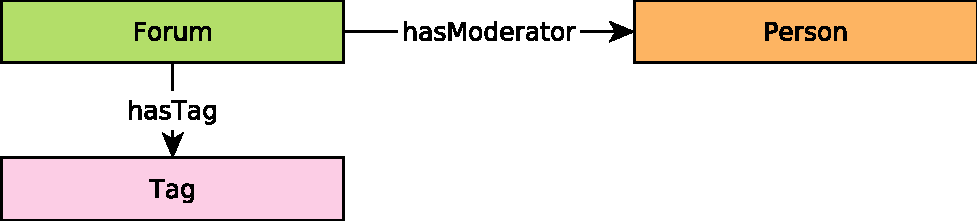
\includegraphics[scale=\patternscale,margin=0cm .2cm]{patterns/interactive-update-04} \tabularnewline \hline
%
	desc. & Add a \emph{Forum} \textbf{node}, connected to the network by 2 possible
\textbf{edge} types.
 \\ \hline
%
	
		params &
		\innerCardVSpace{\begin{tabularx}{\attributeCardWidth}{|>{\paramNumberCell}c|>{\varNameCell}M|>{\typeCell}m{\typeWidth}|Y|} \hline
		$\mathsf{1}$ & Forum.id
 & ID
 & \texttt{forumId}
 \\ \hline
		$\mathsf{2}$ & Forum.title
 & String
 & \texttt{forumTitle}
 \\ \hline
		$\mathsf{3}$ & Forum.creationDate
 & DateTime
 & \texttt{creationDate}
 \\ \hline
		$\mathsf{4}$ & Forum-hasModerator-\textgreater{}Person.id
 & ID
 & \texttt{moderatorPersonId}
 \\ \hline
		$\mathsf{5}$ & Forum-hasTag-\textgreater{}Tag.id
 & \{ID\}
 & \texttt{tagIds}
 \\ \hline
		\end{tabularx}}\innerCardVSpace \\ \hline
	
%
	
%
	%
	%
	%
	%
\end{tabularx}
\queryCardVSpace

% change \emph back to the old one
\let\emph\oldemph